\chapter{Speed Feedback}
\section{Overview}
The primary consideration of this section is developing and evaluating a speed feedback sub-system for the autonomous `mouse'. A limitation of the current `mouse' design is its inability to monitor the RPM of the wheels, meaning the controller cannot adjust the PWM accounting for a sudden reduction or increase in RPM. A typical example of a RPM-related issue is the descent of the track hill. When descending, it is common for the `mouse' to lose control due to a sudden increase in RPM and the controller's inability to account for this. The proposed solutions must provide reliable and responsive RPM readings. The solutions will be evaluated based on the following criteria: stability, simplicity of integration and cost of implementation.

\section{Design Concepts and Methods}
\subsection{Design D: Hall-Effect Sensor}
Design D (Fig.\ref{fig:hes_theory}) utilises a digital hall-effect sensor to detect the presence of a magnet attached to the `mouse' wheel, outputting a signal based on the presence or absence of a magnetic field. Many hall-effect sensors have an open-drain or open-collector output stage, meaning they can pull the output low but not drive it high, for example Allegro A3213 \cite{MicroSystems_2016}. 

\begin{figure}[H]
    \centering
    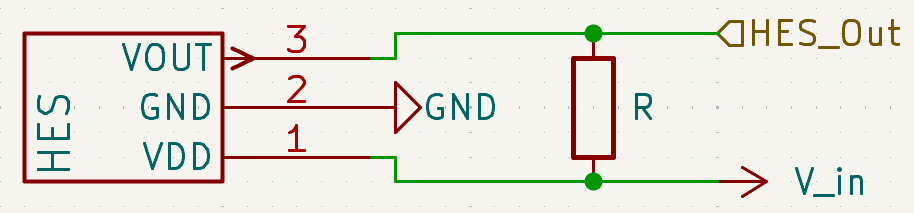
\includegraphics[width=1\textwidth]{circuits/hes_sensor_theory.png}
    \caption[Hall-Effect Sensor with Pull-up Resitor Schematic]{Schematic of a hall-effect sensor circuit with pull-up resistor}
    \label{fig:hes_theory}
\end{figure}

To obtain an observable pulse it is common to use a pull-up resistor between the supply rail and sensor output (Fig.\ref{fig:hes_theory}). This circuit setup results in logic low (0: negative pulse) observed on VOUT when applying a magnetic field and logic high (1: high voltage) when not applying a magnetic field. Typical values for the pull-up resistor (`R') range from \(1\) k\(\Omega\rightarrow50\) k\(\Omega\) depending on required logic levels, speed and current. A smaller `R' value results in a faster response time and an increased current draw when the output is low. A pull-up resistor is critical when interfacing the hall-effect sensor with digital inputs on microcontrollers or logic devices. Without a pull-up resistor, the output may float, resulting in undefined or noisy readings.

\subsection{Design E: IR Optical Sensor}
\begin{figure}[H]
    \centering
    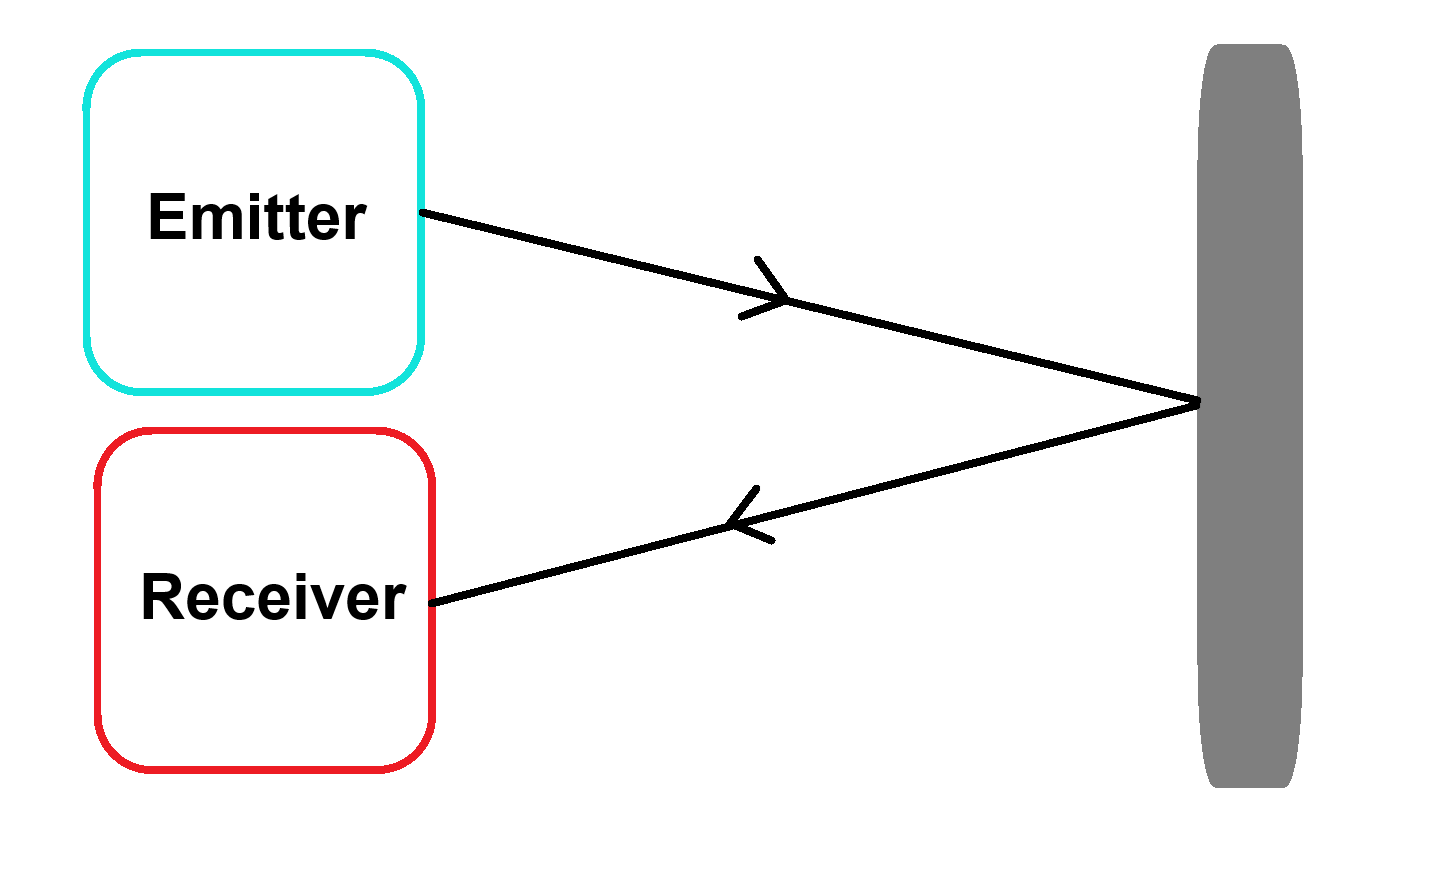
\includegraphics[width=0.6\textwidth]{photos/emitter&receiver.png}
    \caption{Diagram of IR emitter and receiver behaviour}
    \label{fig:opt_theory}
\end{figure}
Design E employs a digital IR emitter and receiver module \cite{Switch_TCRT5000} for detecting the presence of tachometer tape on the `mouse' wheel, outputting a signal based on the presence or absence of IR reflection. The system typically consists of an IR Light Emitting Diode (LED) as the emitter and a phototransistor or photodiode as the receiver. The IR LED emits invisible infrared light toward a target area.

The module utilises a reflective configuration; the emitter and receiver are positioned adjacent facing the target area. When the tachometer tape enters the sensor’s detection zone, it reflects the IR light towards the receiver (Fig.\ref{fig:opt_theory}). The sensor output is then converted from analogue to digital via a comparator or signal conditioning, and the output remains logic low (0: low voltage) when no reflection is detected and switches to logic high (1: high pulse) when a reflection is detected.

\section{Procedures}
Initially, the `mouse' wheel was modified, a \(3\) mm neodymium magnet \cite{RS_2192257} was adhered using hot glue to the outside of the wheel and covered by reflective tachometer tape \cite{RS_8459731} as shown in Fig.\ref{fig:wheel_mag}.

\begin{figure*}[!h]
    \centering
    \begin{subfigure}[t]{0.3\textwidth}
        \centering
        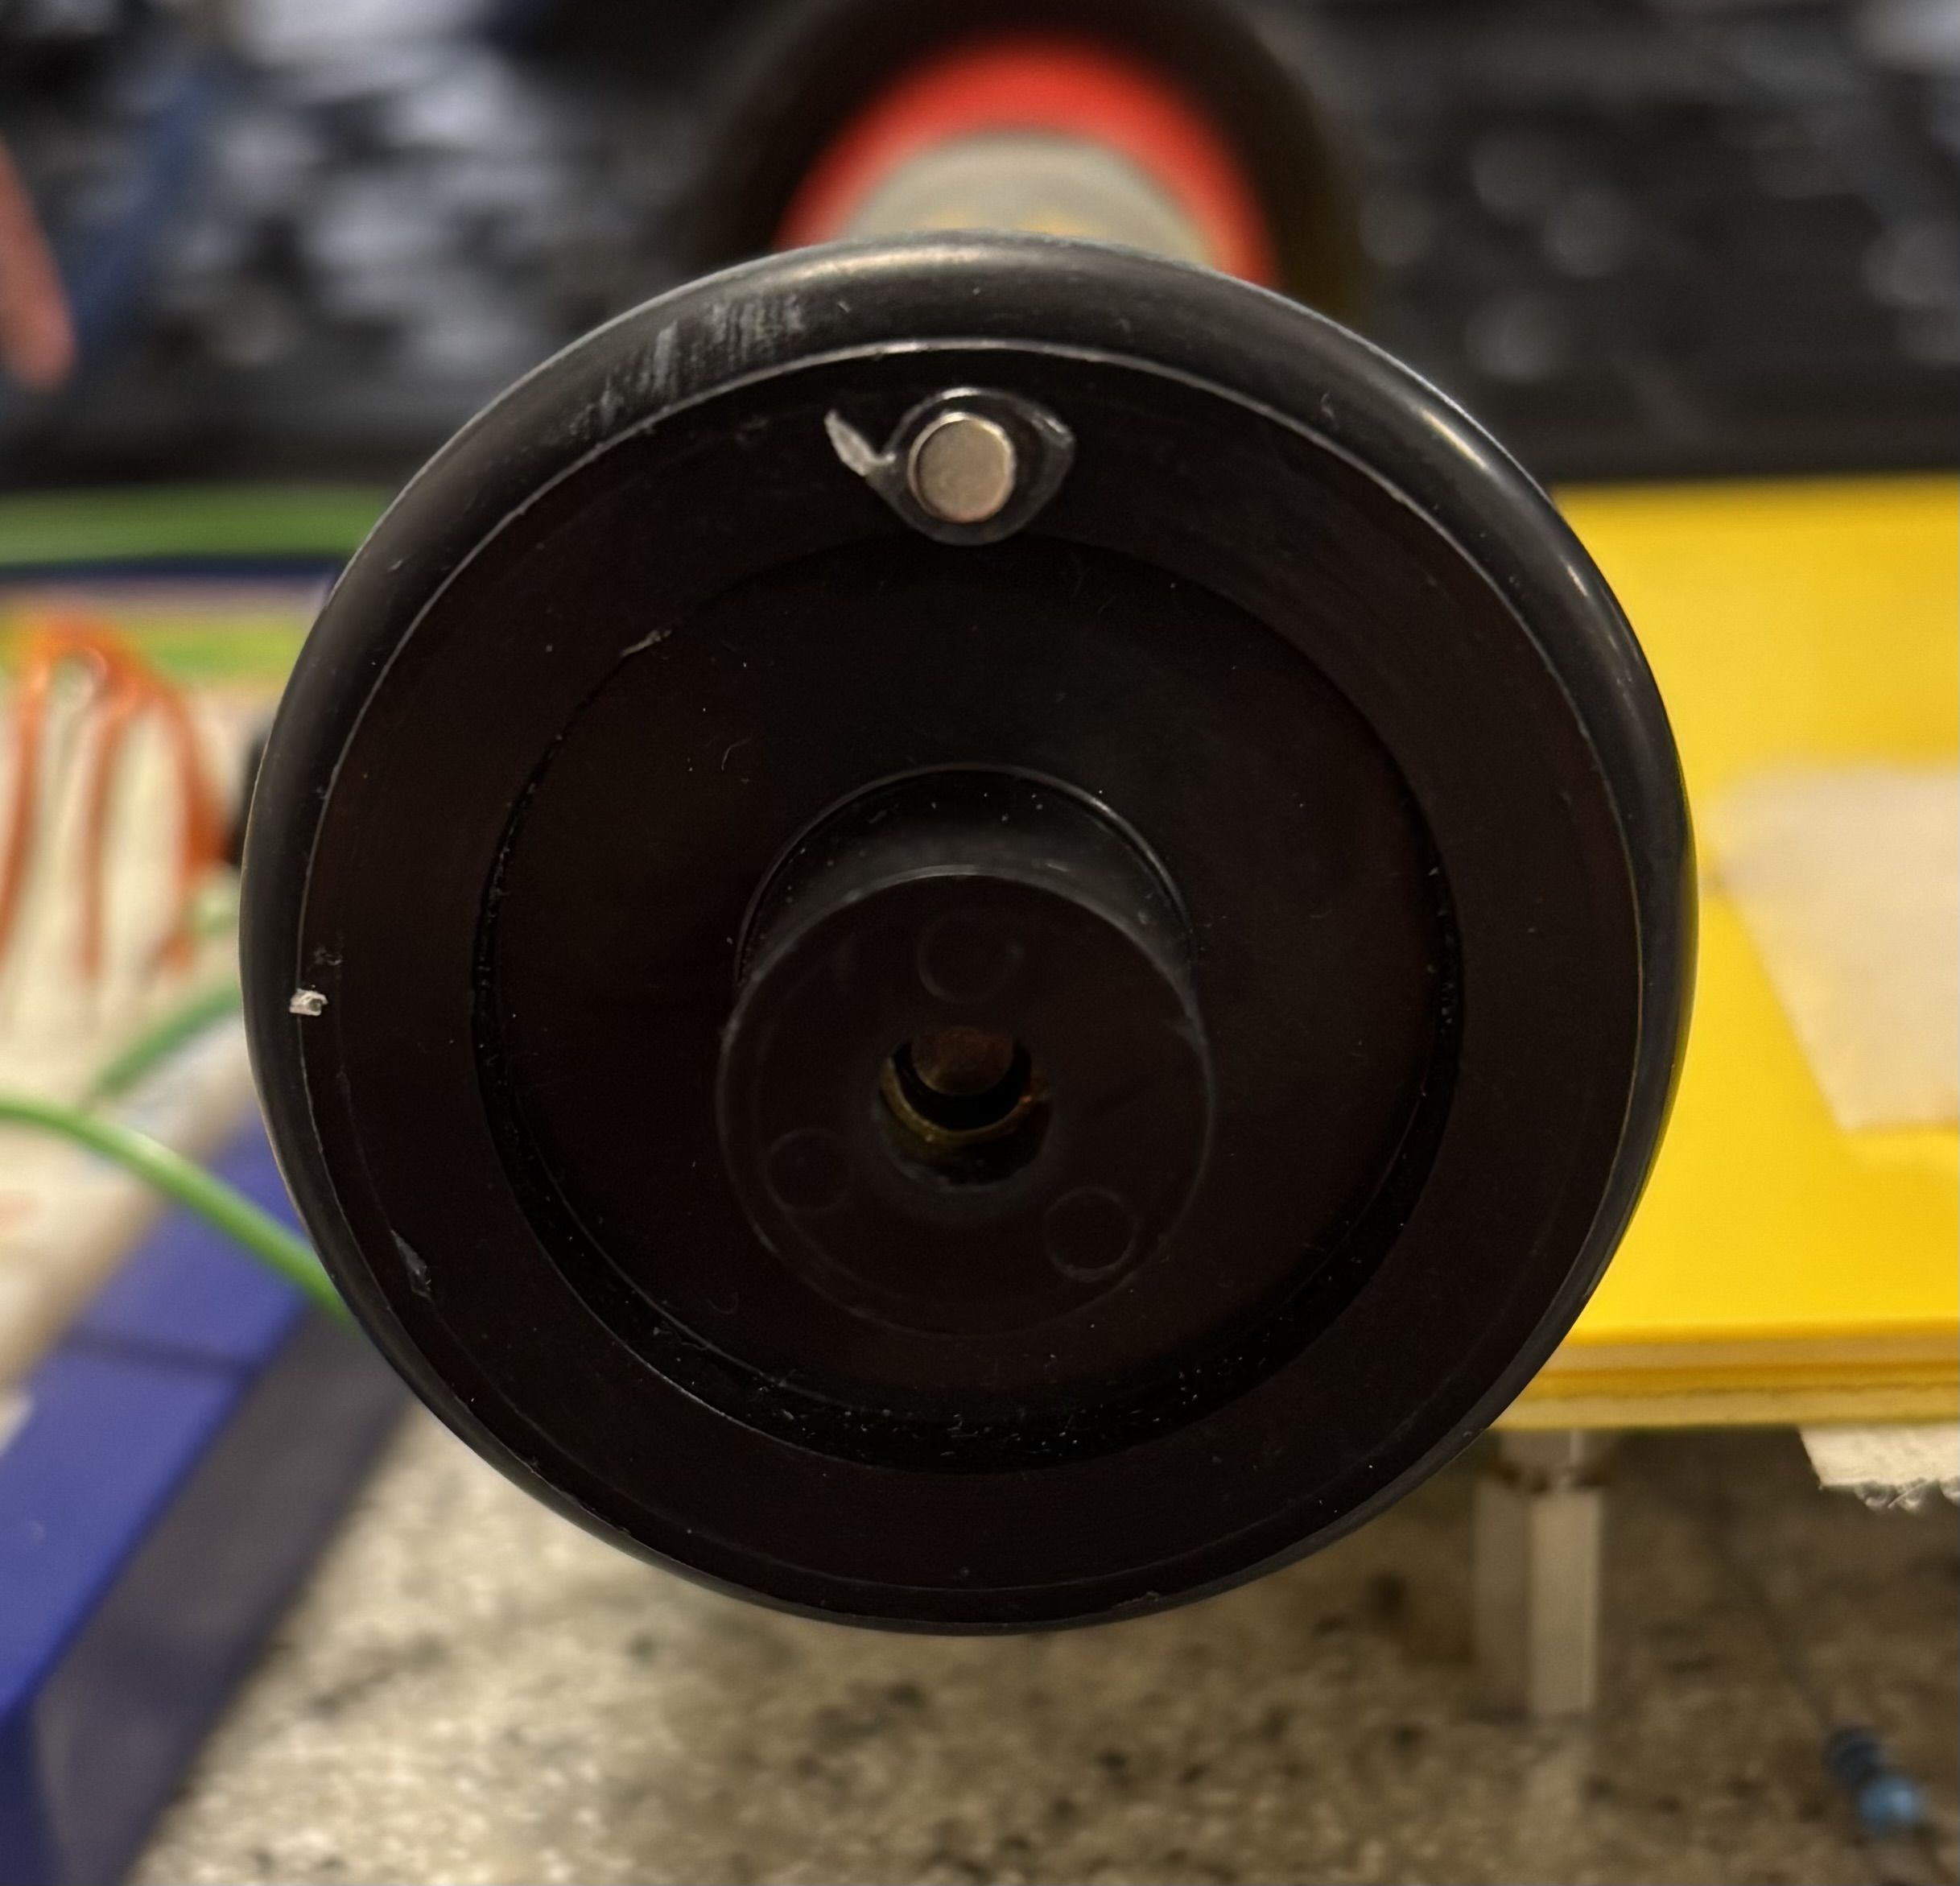
\includegraphics[height=0.8\linewidth]{photos/wheel_2.jpg}
        \caption{}
    \end{subfigure}%
    ~ 
    \begin{subfigure}[t]{0.3\textwidth}
        \centering
        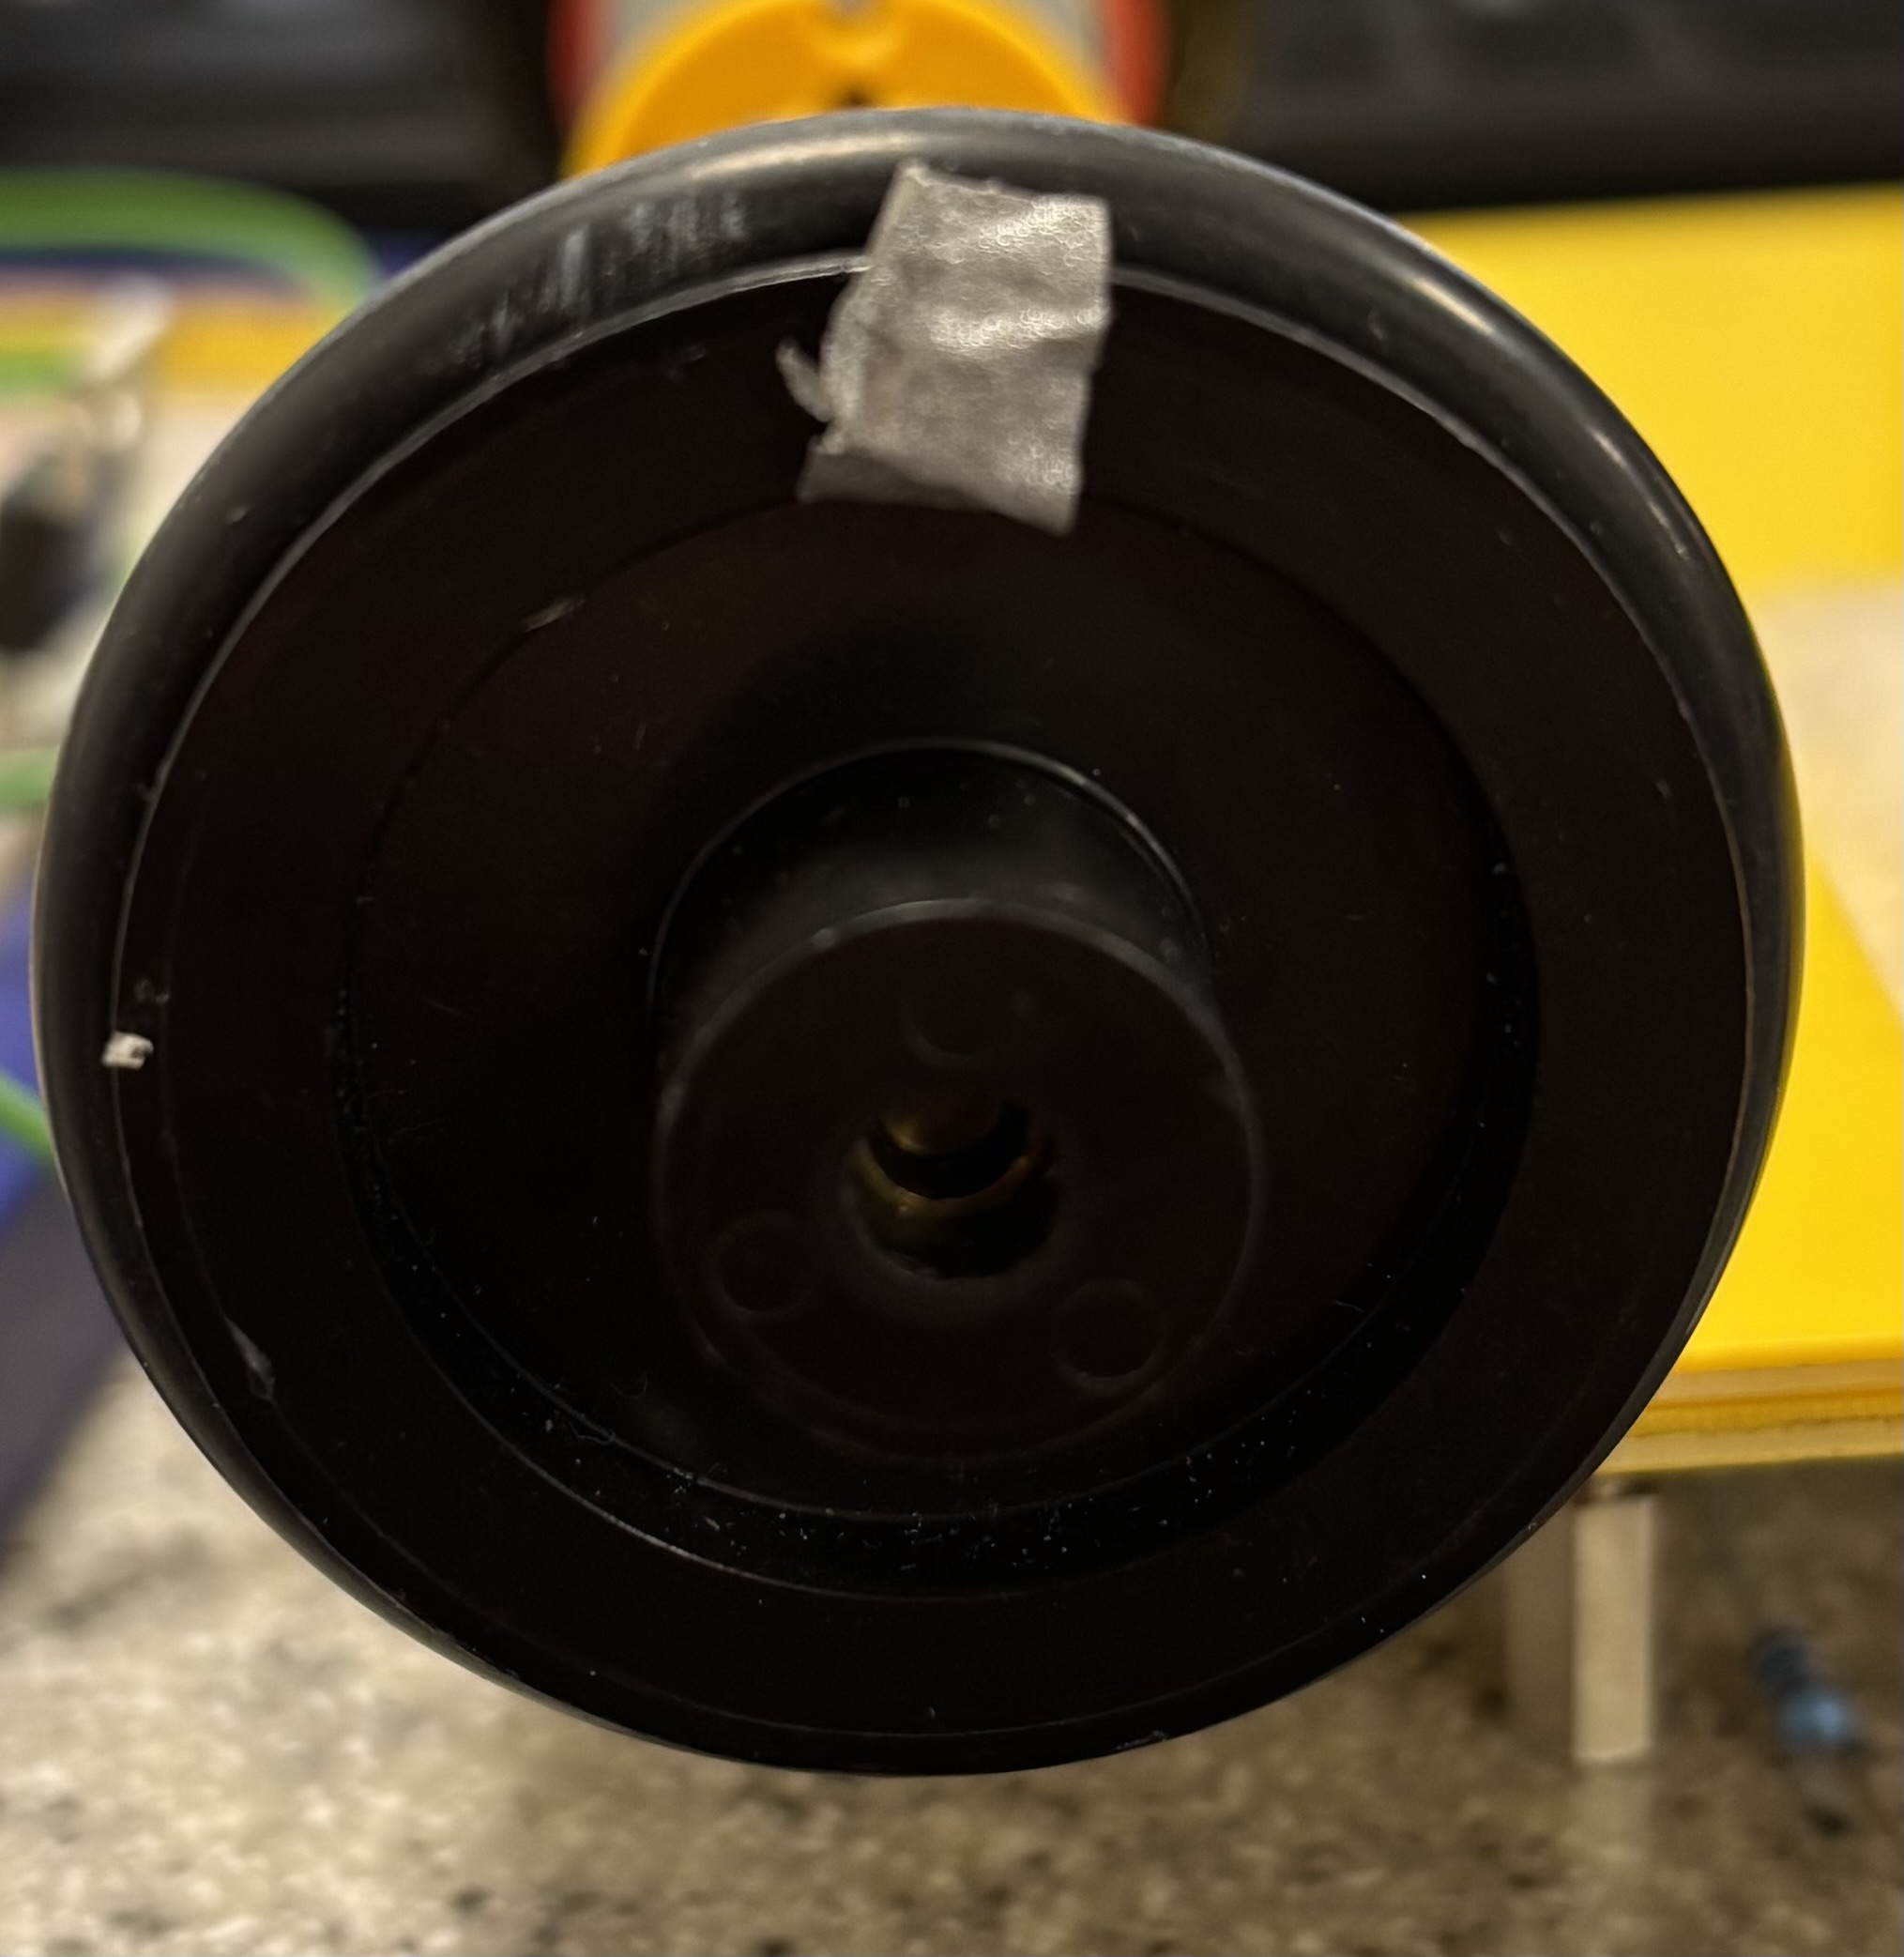
\includegraphics[height=0.8\linewidth]{photos/wheel_1.jpg}
        \caption{}
    \end{subfigure}
    \caption[Photographs of `mouse' wheel]{Photographs of `mouse' wheel: (a) `mouse' wheel with attached magnet (b) `mouse' wheel with tachometer tape over attached magnet}
    \label{fig:wheel_mag}
\end{figure*}

\subsection{Design D: Hall-Effect Sensor}
\label{sec:hes}
\label{sec:4}
Design D was built on a standard RH-32 breadboard reflecting the schematic shown in Fig.\ref{fig:hes_sensor_c}. First, the A3213EUA-T hall-effect sensor \cite{MicroSystems_2016} was placed at the edge of the breadboard. Since A3213EUA-T is an open-drain digital sensor, a \(10\) k\(\Omega\) pull-up resistor is connected from pin 1 (VDD) to pin 3 (VOUT). Second, the Arduino Nano Every was placed into the breadboard over the central channel, the GND, \(+5\) V Arduino supply and digital pin (D2) were connected to the hall-effect sensor as shown in Fig.\ref{fig:hes_sensor_c}. All circuit connections were kept short to maintain signal integrity and reduce the chance of EMI and noise.

\begin{figure}[H]
\centering
    \centering
    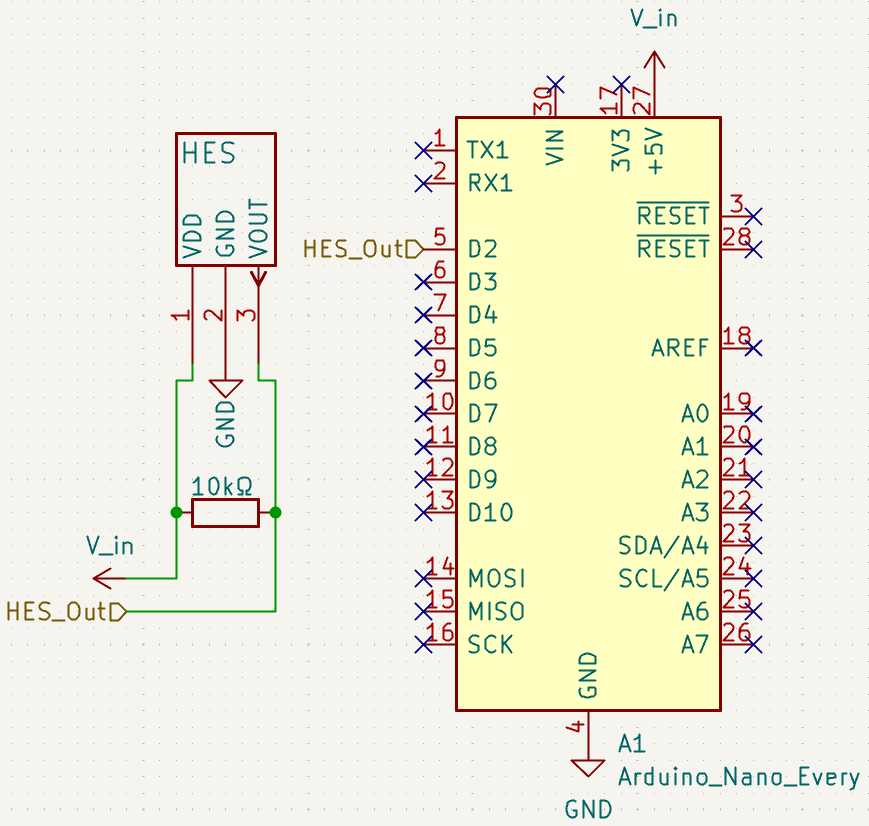
\includegraphics[width=0.7\linewidth]{circuits/hes_sensor.png}
    \caption[Design D: Schematic]{Schematic diagram of Design D; a Hall-effect sensor with \(10\) k\(\Omega\) pull-up resistor}
    \label{fig:hes_sensor_c}
\end{figure}

Finally, an Arduino program was developed and uploaded to the Arduino Nano Every  (Appendix \ref{app:Arduino} Listing \ref{cod:RPM}). The program utilised an interrupt service routine (ISR) to increment a global counter when a pulse was detected; the condition used was `FALLING'. The system recorded the time taken for four consecutive pulses, corresponding to four complete revolutions of the wheel, and subsequently calculated the rotational speed in RPM. The RPM value is then output to the serial interface. This approach allowed for the capturing of precise timestamps on interrupt-triggered events, minimising timing errors associated with polling, and by averaging the RPM calculation over four complete revolutions, the calculated output was a steadier more reliable RPM value.

\newpage
\subsubsection{Testing}
The steps for Testing Design D are as follows:

\begin{enumerate}
    \item The motor terminals \cite{mfa_motor} for the modified `mouse' wheel were connected to the \(6\) V DC range terminals of a KeySight E3631A variable power supply.
    \item The mouse chassis was then placed with the wheel facing the breadboard, magnet and tachometer tape towards the hall-effect sensor. The chassis was then moved till the distance between the sensor and wheel was \(\approx 1\) mm.
    \item The power supply was then turned on and set to a value of \(2\) V, and it was then noted if the hall-effect sensor was behaving as expected and tripping the interrupt correctly. The distance was then increased until the sensor stopped working; this distance was measured with a set of digital vernier callipers. Repeated three times to find an average.
    \item The distance between the sensor and the wheel was reduced back to \(\approx3\) mm (Photo of setup), the motor voltage was then set to \(1.0\) V. The RPM was measured thrice with an AT-6 tachometer, and three concurrent RPM calculated values from the Arduino Serial Monitor. The RPM values were recorded in Excel for later analysis. The voltage was then increased in increments of \(1.0\) V and measurements retaken till the motor voltage reached \(6.0\) V.
    \item The Keysight DSO1014A oscilloscope was connected to Design D, making sure the oscilloscope probe ratio matched the input signal ratio and the probe point was as close as possible to the hall-effect sensor. Channel 1 was connected to the sensor output `VOUT', and the probe reference was connected to GND.
    \item The distance between the sensor and the wheel was set back at \(\approx3\) mm, and motor voltage was set to \(3.0\) V. The steady-state waveform was observed and stored on an external USB as a CSV for later analysis in Excel.
\end{enumerate}

All measurements were taken after a 5-second stabilisation period to minimise transient effects and were conducted at room temperature (approximately 22°C). The oscilloscope output was imported into Excel and used to generate graphs for analysing rise and fall time. The tachometer and Arduino RPM readings were tabulated and averaged, statistical analysis was conducted to review the absolute error.

\subsection{Design E: Optical Feedback}
\label{sec:5}
\begin{figure}[H]
    \centering
    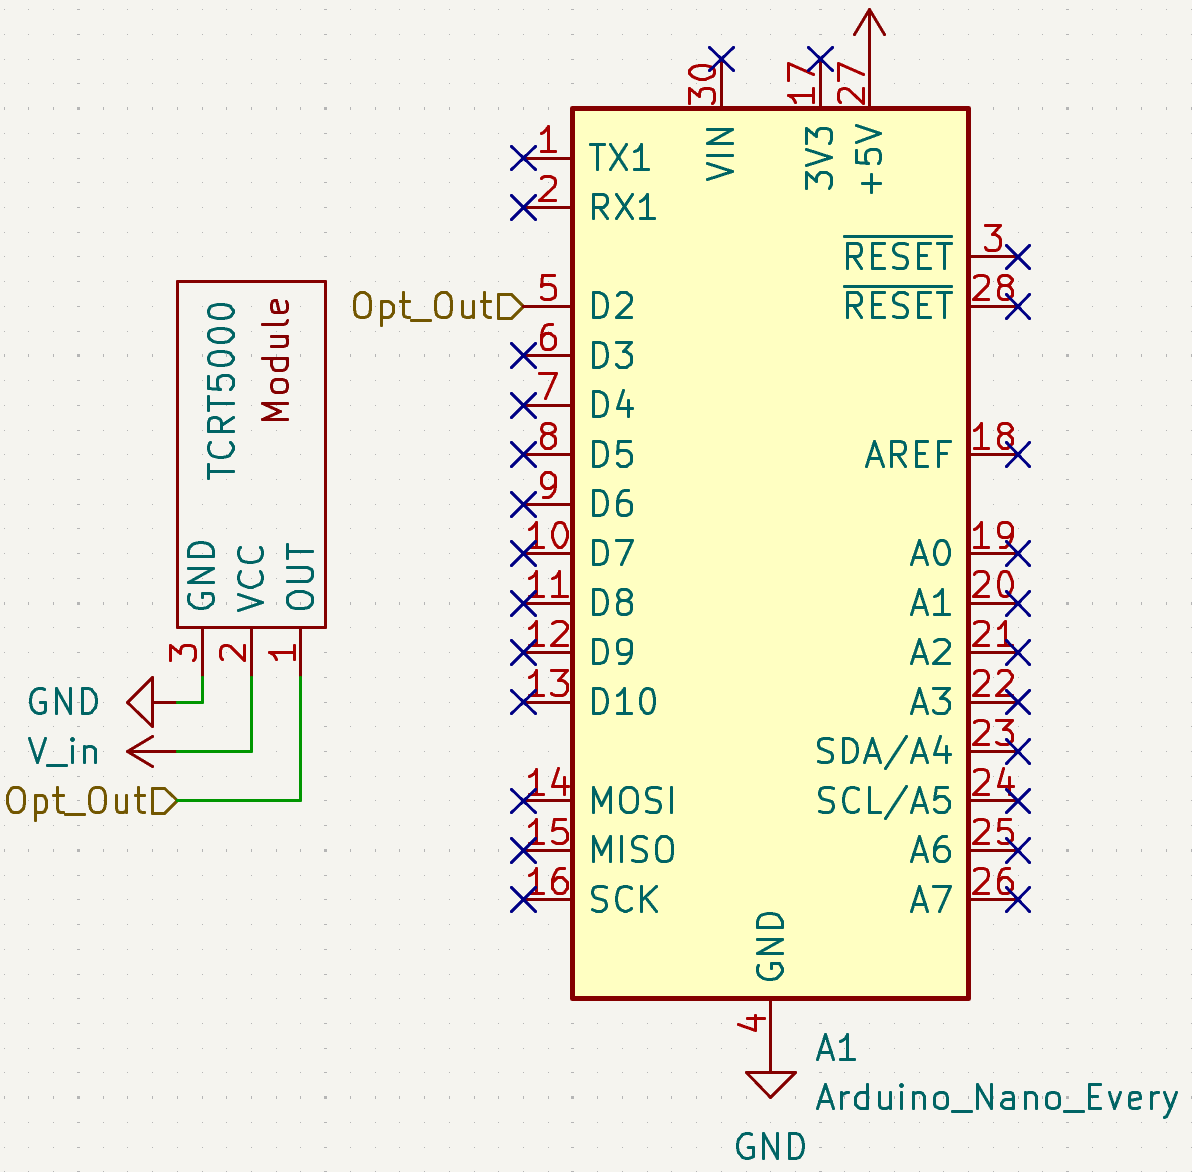
\includegraphics[width=0.75\textwidth]{circuits/opt_sensor.png}
    \caption[Design E: Schematic]{Schematic diagram of Design E; a Optical sensor module direct connections to Arduino Nano Every.}
    \label{fig:opt_sensor_c}
\end{figure}

Design E utilised a TCRT5000 optical sensing module \cite{Switch_TCRT5000}, made by Switch Electronics. Using breadboard jumper cables, the module was directly connected to the Arduino Nano Every as per the schematic Fig.\ref {fig:opt_sensor_c}. The RPM code (Appendix \ref{app:Arduino} Listing \ref{cod:RPM}) was re-uploaded to the Arduino Nano Every with the ISR updated to look for the `RISING' condition.

\subsubsection{Testing}
The testing method for Design D followed the same procedure as outlined in Section \ref{sec:hes}, except for the sensor being placed \(\approx5\) mm away during testing when distances are stated. All measurements were taken under the same conditions and analysed accordingly.


\newpage
\section{Results}
\subsection{Design D: Hall-Effect Sensor}
The average maximum distance observed before failure was \(\approx3\) mm (Appendix \ref{app:data} Table \hyperref[tab:A.5]{A.5}).

As summarised in Table \ref{tab:HES_VoltRPM} the hall-effect sensor Arduino RPM values are consistent with the tachometer reference values, with deviation remaining within \(\pm 0.54\%\). This variation in values is due to the integer nature of the Arduino RPM calculation, reducing potential accuracy.

\begin{table}[H]
    \centering
    \caption[Design D: RPM Measurements]{Hall-effect sensor Arduino Calculated RPM compared to measured Tachometer RPM at varying voltages from \(1.0\rightarrow6.0\) V (Appendix \ref{app:data} Table \hyperref[tab:A.4]{A.4}). The tachometer took readings at an accuracy of 4 s.f. and the Arduino calculated RPM values were set to be integers.}
    \label{tab:HES_VoltRPM}
    \begin{tabular}{|c||c|c|c|c|}\hline
    &\multicolumn{2}{|c|}{RPM} &  &\\\hline
    Voltage (V)&Tachometer Average&Arduino Average&Absolute Error &Percentage Error\\ \hline 
    1.0&131.3&132 &-0.7&0.54\\ \hline
    2.0&350.3&350 &0.3&0.10\\\hline
    3.0&566.0&566 &0.0&0.00\\\hline
    4.0&759.3&759 &0.2&0.03\\\hline
    5.0&982.9&983 &-0.1&0.01\\\hline
    6.0&1176&1175 &0.0&0.00\\\hline\end{tabular}  
\end{table}

Observing and analysing the output waveforms from the A3213EUA-T on the DSO1014A oscilloscope (Fig.\ref{fig:hes_osc}) when triggered, the fall time of the signal to a steady state is \(\approx0.04\) \(\mu\)s and the signal has a rise time of \(\approx2.25\) \(\mu\)s to steady state. The signal has a clean edge with no oscillation, indicating a strong digital signal.

\begin{figure*}[h!]
    \centering
    \begin{subfigure}{0.8\textwidth}
        \centering
        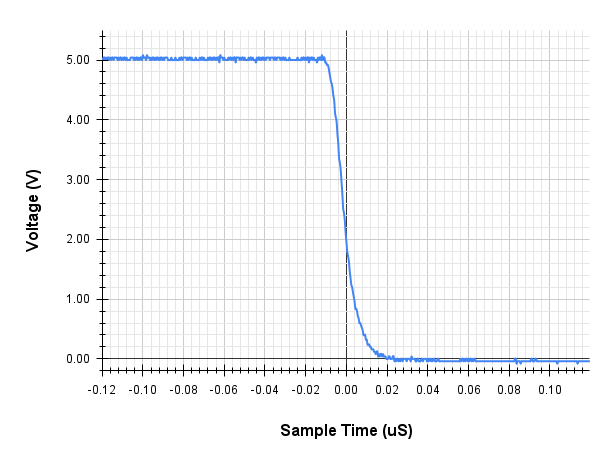
\includegraphics[width=1\linewidth]{graphs/hes_f_osciliscope.png}
        \caption{}
    \end{subfigure}
    \begin{subfigure}{0.8\textwidth}
        \centering
        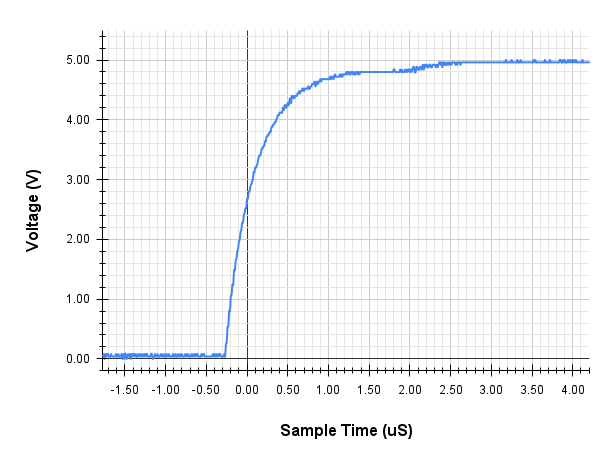
\includegraphics[width=1\linewidth]{graphs/hes_r_osciliscope.png}
        \caption{}
    \end{subfigure}
    \caption[Design D: Oscilliscope Rise and Fall]{A3213EUA-T output waveform from a DSO1014A oscilloscope, split into rise and fall conditions: (a) Falling signal edge (b) Rising signal edge}
    \label{fig:hes_osc}
\end{figure*}

\subsubsection{Cost of Implementation}

\begin{table}[H]
\centering
\caption{Alphabetically Ordered Estimated Component Costs for Design D}
\label{tab:design_d_cost}
\begin{tabularx}{\linewidth}{|l|X|X|X|}
\hline
\textbf{Component} & \textbf{Quantity} & \textbf{Unit Price (£)} & \textbf{Total Price (£)}\\ \hline
10kΩ Through-Hole Resistor \cite{rs_10kresistor}& 1 & 0.07 & 0.07\\ \hline
Allegro A1101EUA-T Hall-Effect Sensor IC \cite{MicroSystems_2016}& 1 & 0.69 & 0.69\\ \hline
Neodymium Magnet 10mm x 3mm \cite{RS_2192257} & 1 & 0.11 & 0.11\\ \hline\hline
\textbf{Total Estimated Cost} & & & \textbf{£0.87}\\ \hline
\end{tabularx}
\end{table}

Table \ref{tab:design_d_cost} details the individual components required to implement Design E, alongside their quantities, suppliers and unit costs based on UK-sourced pricing at the time of writing.

\newpage
\subsection{Design E: Optical Feedback}
The average maximum distance observed before failure was \(\approx13\) mm (Appendix \ref{app:data} Table \hyperref[tab:A.7]{A.7}).

As summarised in Table \ref{tab:Opt_VoltRPM} the optical sensor Arduino RPM values are consistent with the tachometer reference values, with deviation remaining within \(\pm 0.75\%\). This variation in values is due to the integer nature of the Arduino RPM calculation, reducing potential accuracy.

\begin{table}[H]
    \centering
\caption[Design E: RPM Measurements]{Optical sensor Arduino calculated RPM compared to measured Tachometer RPM at varying voltages from \(1.0\rightarrow6.0\) mm (Appendix \ref{app:data} Table \hyperref[tab:A.6]{A.6}). The tachometer took readings at an accuracy of 4 s.f. and the Arduino calculated RPM values were set to be integers.}
\label{tab:Opt_VoltRPM}
    \begin{tabular}{|c||c|c|c|c|}\hline
    &\multicolumn{2}{|c|}{RPM} &  &\\\hline
    Voltage (V)&Tachometer Average&Arduino Average&Absolute Error &Percentage Error\\ \hline 
    1.0&128.6&129&-0.4&0.29\\ \hline
    2.0&352.6&350&2.6&0.75\\\hline
    3.0&565.1&567&-1.9&0.34\\\hline
    4.0&760.2&760&0.2&0.03\\\hline
    5.0&982.9&983&-0.1&0.01\\\hline
    6.0&1174&1174&0.0&0.00\\\hline\end{tabular}  
\end{table}

Observing and analysing the output waveforms from the TCRT5000 sensor module on the DSO1014A oscilloscope (Fig.\ref{fig:opt_osc}) when triggered, the fall time of the signal is \(\approx0.045\) \(\mu\)s and the signal has a rise time of \(\approx0.045\) \(\mu\)s. The signal has oscillations when changing state, indicating a weaker digital signal.

\begin{figure*}[h!]
    \centering
    \begin{subfigure}{0.8\textwidth}
        \centering
        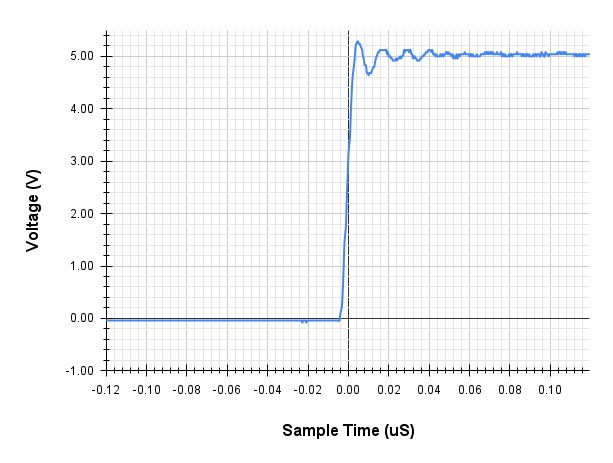
\includegraphics[width=1\linewidth]{graphs/opt_r_osciliscope.png}
        \caption{}
    \end{subfigure}
    \begin{subfigure}{0.8\textwidth}
        \centering
        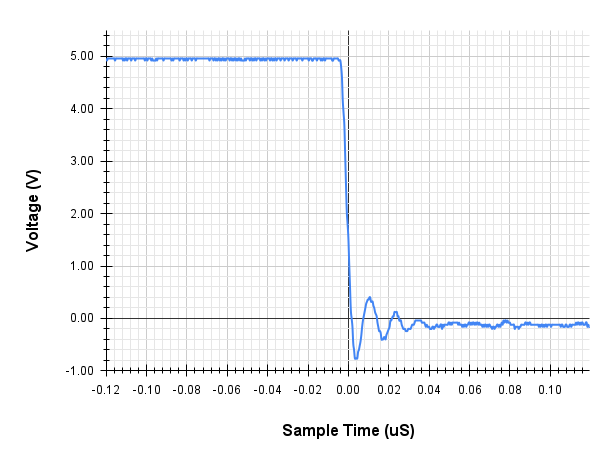
\includegraphics[width=1\linewidth]{graphs/opt_f_osciliscope.png}
        \caption{}
    \end{subfigure}
    \caption[Design E: Oscilliscope Rise and Fall]{Hall-effect sensor output waveform from a DSO1014A oscilloscope, split into rise and fall conditions: (a) Rising signal edge (b) Falling signal edge}
    \label{fig:opt_osc}
\end{figure*}

\subsubsection{Cost of Implementation}
\begin{table}[H]
\centering
\caption{Alphabetically Ordered Estimated Component Costs for Design E}
\label{tab:design_e_cost}
\begin{tabularx}{\linewidth}{|l|X|X|X|}
\hline
\textbf{Component}                                   & \textbf{Quantity} & \textbf{Unit Price (£)} & \textbf{Total Price (£)} \\ \hline
Infrared Line Tracking Sensor Module (TCRT5000) \cite{Switch_TCRT5000} & 1 & 1.37  & 1.37\\ \hline
RS Reflective Tachometer Tape \cite{RS_8459731}& 1 & 0.87 & 0.87\\ \hline\hline
\textbf{Total Estimated Cost}                        &   &       & \textbf{£2.24} \\ \hline
\end{tabularx}
\end{table}

Table \ref{tab:design_e_cost} details the individual components required to implement Design E, alongside their quantities, suppliers and unit costs based on UK-sourced pricing at the time of writing.

\newpage
\section{Discussion}
This section evaluates two design solutions proposed to facilitate the addition of a speed feedback system to improve the control loop currently implemented in the `mouse' design. Both designs worked as expected and provide a reliable RPM value. Design D (HES) may be a more appropriate solution as it provides a potential learning opportunity in magnetic sensing and related components, and not a plug-and-play module. 

\subsubsection{Design Performance}
Design D provided a consistent and reliable RPM. However, the HES and trigger magnet must be within 3mm (Appendix \ref{app:equip&test} Figure \ref{fig:hes_distance_measurements}) of each other to provide accurate detection.

Design E provided a stable and accurate RPM. To avoid false positives, the distance between the sensor and reflective tape should be no more than 5mm (Appendix \ref{app:equip&test} Figure \ref{fig:opt_distance_measurements}). In addition, it is recommended that the wheel's surface be non-reflective.

\subsubsection{Complexity}
Both Design D and E would be easy to introduce into the `mouse' platform, with various levels of documentation to assist in assembly. However, it is easier to position the HES sensor than the optical module. On the other hand, Design D requires chassis modification in the addition of a magnet to the wheel.

\subsubsection{Cost}
When comparing the cost of implementation, Design D is the preferable option, only introducing a cost estimate per `mouse' of £0.87, which is £1.37 less than the cost of Design E's implementation, which is £2.24. However, these costs do not account for the potential technician time to modify the `mouse' chassis.

\subsubsection{Further Investigations}
Additional research should be conducted on incorporating the RPM measurement into a working ‘mouse’ control loop. In addition, a potential investigation could be conducted on creating an IR optical sensor circuit instead of a pre-fabricated module.

\subsubsection{Recommendations}
Both Design D and E could be used to great effect on the `mouse' platform. However, I suggest Design D as the most appropriate option, as it provides learning opportunities and reliable, cost-effective RPM measurements.